\section{拉普拉斯变换}

\subsection{从傅里叶变换到拉普拉斯变换}

\begin{BoxDefinition}[拉普拉斯变换]
    为满足函数的绝对可积条件求解傅里叶变换,可用一个衰减因子$e^{-\sigma t}$($\sigma$为实数)乘信号$f(t)$使得$f(t)e^{-\sigma}$在$t\rightarrow\infty$时信号幅度趋于$0$,此时$f(t)e^{-\sigma}$的傅里叶变换存在,即
    \begin{Equation}
        F_b(\sigma+\mathrm{j}\omega) = \mathscr{F}\left[f(t)e^{-\sigma t}\right] = \int_{-\infty}^{\infty} f(t)e^{-(\sigma+\mathrm{j}\omega)t}dt
    \end{Equation}
    其傅里叶逆变换为
    \begin{Equation}
        f(t)e^{-\sigma} = \frac{1}{2\pi} \int_{-\infty}^{\infty} F_b(\sigma + \mathrm{j}\omega)e^{\mathrm{j}\omega t}d\omega
    \end{Equation}
    即
    \begin{Equation}
        f(t) = \frac{1}{2\pi} \int_{-\infty}^{\infty}F_b(\sigma+\mathrm{j}\omega)e^{(\sigma+\mathrm{j}\omega)t}d\omega
    \end{Equation}
    令$s=\sigma+\mathrm{j}\omega$,$d\omega = \frac{ds}{\mathrm{j}}$,则有
    \begin{Equation}
        F_b(s) = \int_{-\infty}^{\infty}f(t)e^{-st}dt
    \end{Equation}
    \begin{Equation}
        f(t) = \frac{1}{2\pi \mathrm{j}}\int_{\sigma-\mathrm{j}\infty}^{\sigma+\mathrm{j}\infty} F_b(s)e^{st}ds
    \end{Equation}
    $F_b(s)$称为$f(t)$的双边拉普拉斯变换,又称为象函数;

    $f(t)$称为$F_b(s)$的双边拉普拉斯逆变换,又称为原函数。
\end{BoxDefinition}

\subsection{收敛域}

\begin{BoxDefinition}[收敛域]
    只有适当的$\sigma$值才能使得积分收敛,信号$f(t)$的拉普拉斯变换存在,其中$\sigma$的取值范围称为$F_b(s)$的收敛域。
\end{BoxDefinition}

\begin{BoxFormula}[指数函数因果信号的拉普拉斯变换]
    指数函数因果信号
    \begin{Equation}
        f(t) = e^{\alpha t}\varepsilon(t)
    \end{Equation}
    拉普拉斯变换
    \begin{Equation}
        \begin{aligned} F_b(s) = \int_{0}^{\infty} e^{\alpha t}e^{-st}dt = \left.\frac{e^{-(s-\alpha)t}}{-(s-\alpha)}\right|_{0}^{\infty} &= \frac{1}{s-\alpha}\left[1-\lim\limits_{t\rightarrow\infty} e^{-(\sigma-\alpha)t}e^{-\mathrm{j}\omega t}\right] \\
            &= \left\{\begin{aligned}
                \frac{1}{s-\alpha} & , & \mathrm{Re}\left[s\right] = \sigma > \alpha \\
                \text{不定} & , & \sigma = \alpha \\
                \text{无界} & , & \sigma < \alpha
            \end{aligned}
            \right.
        \end{aligned}
    \end{Equation}
    故收敛域如下图
    \begin{Figure}[指数函数因果信号的拉氏变换收敛域]
        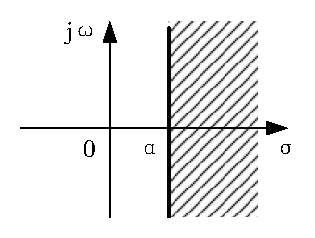
\includegraphics[width=40mm]{visio/5.1.pdf}
    \end{Figure}
\end{BoxFormula}

\begin{BoxFormula}[指数函数反因果信号的拉普拉斯变换]*
    指数函数反因果信号
    \begin{Equation}
        f(t) = e^{\beta t}\varepsilon(-t)
    \end{Equation}
    拉普拉斯变换
    \begin{Equation}
        \begin{aligned} F_b(s) = \int_{-\infty}^{0} e^{\beta t}e^{-st}dt = \left.\frac{e^{-(s-\beta)t}}{-(s-\beta)}\right|_{-\infty}^{0} &= \frac{1}{-(s-\beta)}\left[1-\lim\limits_{t\rightarrow-\infty} e^{-(\sigma-\beta)t}e^{-\mathrm{j}\omega t}\right] \\
            &= \left\{\begin{aligned}
                \text{无界} & , & \mathrm{Re}\left[s\right] = \sigma > \beta \\
                \text{不定} & , & \sigma = \beta \\
                \frac{1}{-(s-\beta)} & , & \sigma < \beta
            \end{aligned}
            \right.
        \end{aligned}
    \end{Equation}
    故收敛域如下图
    \begin{Figure}[指数函数反因果信号的拉氏变换收敛域]
        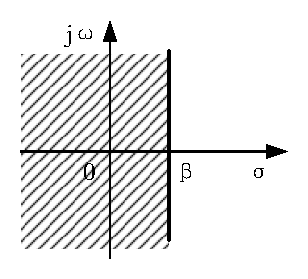
\includegraphics[width=40mm]{visio/5.2.pdf}
    \end{Figure}
\end{BoxFormula}

\begin{BoxFormula}[双边指数函数信号的拉普拉斯变换]
    双边指数函数信号
    \begin{Equation}
        f(t) = \left\{\begin{aligned}
            e^{\beta t} & , & t<0\\
            e^{\alpha t} & , & t>0
        \end{aligned}
        \right.
    \end{Equation}
    由\xref{fml:指数函数因果信号的拉普拉斯变换}和\xref{fml:指数函数反因果信号的拉普拉斯变换}可知,其拉普拉斯变换为
    \begin{Equation}
        F_b(s) = \frac{1}{s-\alpha} + \frac{1}{-(s-\beta)} \quad , \quad \alpha < \mathrm{Re}\left[s\right] = \sigma < \beta
    \end{Equation}
    故收敛域如下图
    \begin{Figure}[双边指数函数信号的拉氏变换收敛域]
        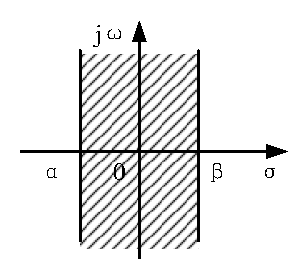
\includegraphics[width=40mm]{visio/5.3.pdf}
    \end{Figure}
\end{BoxFormula}

双边拉氏变换必须写出收敛域,因为不同原函数对应的象函数可能相同,但收敛域不同。

\subsection{单边拉氏变换}

\begin{BoxDefinition}[单边拉普拉斯变换]*
    设信号的初始时刻为坐标原点,此时在$t<0$时$f(t)=0$,拉普拉斯变换为
    \begin{Equation}
        F(s) = \int_{0_{-}}^{\infty} f(t)e^{-st}dt
    \end{Equation}
    \begin{Equation}
        f(t) = \left[\frac{1}{2\pi\mathrm{j}}\int_{\sigma-\mathrm{j}\infty}^{\sigma+\mathrm{j}\infty}F(s)e^{st}ds\right]\varepsilon(t)
    \end{Equation}
    简记为
    \begin{Equation}
        F(s) = \mathscr{L}\left[f(t)\right]
    \end{Equation}
    或
    \begin{Equation}
        f(t) \longleftrightarrow F(s)
    \end{Equation}
    其收敛域一定是$\mathrm{Re}\left[s\right]>\alpha$,可以省略。
\end{BoxDefinition}

\subsection{常见函数的拉普拉斯变换}

\begin{BoxFormula}[冲激函数的拉普拉斯变换]
    冲激函数的拉普拉斯变换\footnote{本课程主要讨论单边拉普拉斯变换,若无特殊说明均为单边}为
    \begin{Equation}
        \delta(t) \longleftrightarrow \int_{0_{-}}^{\infty} \delta(t) e^{-st}dt = 1
    \end{Equation}
\end{BoxFormula}

\begin{BoxFormula}[指数函数的拉普拉斯变换]
    指数函数的拉普拉斯变换为
    \begin{Equation}
         e^{s_0t} \longleftrightarrow \frac{1}{s-s_0} \quad , \quad \sigma > \mathrm{Re}\left[s_0\right]
    \end{Equation}
\end{BoxFormula}

\begin{BoxFormula}[阶跃函数的拉普拉斯变换]
    阶跃函数的拉普拉斯变换为
    \begin{Equation}
         \varepsilon(t) \longleftrightarrow \frac{1}{s} \quad , \quad \sigma > 0
    \end{Equation}
    $1$的拉普拉斯变换也为$\frac{1}{s}$。
\end{BoxFormula}

\begin{BoxFormula}[余弦函数的拉普拉斯变换]
    余弦函数的拉普拉斯变换为
    \begin{Equation}
         \cos \omega_0 t = \frac{1}{2}(\e^{\mathrm{j}\omega_0 t}+e^{-\mathrm{j}\omega_0 t}) \longleftrightarrow \frac{s}{s^2+\omega_0^2}
    \end{Equation}
\end{BoxFormula}

\begin{BoxFormula}[正弦函数的拉普拉斯变换]
    正弦函数的拉普拉斯变换为
    \begin{Equation}
         \sin \omega_0 t = \frac{1}{\mathrm{j}2}(\e^{\mathrm{j}\omega_0 t}-e^{-\mathrm{j}\omega_0 t}) \longleftrightarrow \frac{\omega_0}{s^2+\omega_0^2}
    \end{Equation}
\end{BoxFormula}

\begin{BoxFormula}[周期信号的拉普拉斯变换]
    周期信号的拉普拉斯变换为
    \begin{Equation}
         F_T(s) = \int_{0}^{\infty} f_T(t)e^{-st}dt = \sum\limits_{n=0}^{\infty} \int_{nT}^{(n+1)T} f_T(t)e^{-st}dt
    \end{Equation}
    令$t=t+nT$,则
    \begin{Equation}
        \sum\limits_{n=0}^{\infty}e^{-nsT}\int_{0}^{T}f_T(t)e^{-st}dt = \frac{1}{1-e^{-sT}}\int_{0}^{T} f_T(t)e^{-st}dt
    \end{Equation}
    当$f_T(t)=\delta_T(t)$时,有
    \begin{Equation}
        \delta_T(t) \longleftrightarrow \frac{1}{1-e^{-sT}}    
    \end{Equation}
\end{BoxFormula}

\subsection{单边拉氏变换与傅里叶变换的关系}

\begin{BoxProperty}[单边拉氏变换与傅里叶变换的关系]
    为保证积分限一致,讨论该关系的前提是$f(t)$是因果信号。

    单边拉氏变换
    \begin{Equation}
        F(s) = \int_{0}^{\infty} f(t)e^{-st} dt \quad , \quad \mathrm{Re}\left[s\right]>\sigma_0
    \end{Equation}
    傅里叶变换
    \begin{Equation}
        F(\mathrm{j}\omega) = \int_{-\infty}^{\infty} f(t)e^{-\mathrm{j}\omega t} dt
    \end{Equation}

    当$\sigma_0<0$时,收敛域包含$s=\mathrm{j}\omega$,因此在$s=\mathrm{j}\omega$处满足
    \begin{Equation}
        F(s) = \int_{0}^{\infty} f(t)e^{-\mathrm{j}\omega t} dt = F(\mathrm{j}\omega)
    \end{Equation}
    当$\sigma_0=0$时,收敛域边界为$\mathrm{j}\omega$轴,此时
    \begin{Equation}
        F(\mathrm{j}\omega) = \lim\limits_{\sigma\rightarrow 0} F(s)
    \end{Equation}

    当$\sigma_0>0$时,$F(\mathrm{j}\omega)$不存在
\end{BoxProperty}

对于$\sigma_0 = 0$的情况给出一个例子,例如$f(t)=\varepsilon(t)\longleftrightarrow \frac{1}{s}\quad(\sigma>0)$,此时
\begin{Equation}
    F(\mathrm{j}\omega) = \lim\limits_{\sigma\rightarrow 0} = \lim\limits_{\sigma\rightarrow 0}\frac{1}{\sigma + \mathrm{j}\omega} = \lim\limits_{\sigma\rightarrow 0}\frac{\sigma}{\sigma^2 + \omega^2} + \lim\limits_{\sigma\rightarrow 0}\frac{-\mathrm{j}\omega}{\sigma^2 + \omega^2}
\end{Equation}
其中易知$\lim\limits_{\sigma\rightarrow 0}\frac{-\mathrm{j}\omega}{\sigma^2 + \omega^2}=\frac{1}{\mathrm{j}\omega}$,而$\lim\limits_{\sigma\rightarrow 0}\frac{\sigma}{\sigma^2 + \omega^2}$需要讨论$\omega$

$\omega\neq 0$时,$\lim\limits_{\sigma\rightarrow 0}\frac{\sigma}{\sigma^2 + \omega^2}=0$;

$\omega=0$时,根据狄拉克定义,$\delta(t)$可以等价为

\begin{Equation}
    \delta(t)= \lim\limits_{a\rightarrow 0_{+}} \frac{1}{\pi}\frac{a}{a^2+x^2}
\end{Equation}

因此

\begin{Equation}
    \lim\limits_{\sigma\rightarrow 0}\frac{\sigma}{\sigma^2 + \omega^2} = \pi\delta(t)
\end{Equation}

即

\begin{Equation}
    F(\mathrm{j}\omega) = \pi \delta(\omega) + \frac{1}{\mathrm{j}\omega}
\end{Equation}

